\documentclass[a4paper]{article}

% Packages
\usepackage{listings}
\usepackage{color}
\usepackage[utf8]{inputenc}
\usepackage{listingsutf8}
\usepackage{graphicx}
\usepackage{epstopdf}
\usepackage{fancyhdr}
\usepackage[T1]{fontenc}
\usepackage{pmboxdraw}
\usepackage{parskip}
%\usepackage[top=2cm, bottom=2cm, left=3.5cm, right=2cm]{geometry} % Les marges.
\usepackage[top=2cm, bottom=2cm, left=2cm, right=2cm]{geometry} % Les marges.

\definecolor{mygreen}{rgb}{0,0.6,0}
\definecolor{mygray}{rgb}{0.5,0.5,0.5}
\definecolor{mymauve}{rgb}{0.58,0,0.82}
\definecolor{bggray}{rgb}{0.95, 0.95, 0.95}
\lstset{inputencoding=utf8/latin1}
\lstset{ %
    backgroundcolor=\color{bggray},   % choose the background color; you must add \usepackage{color} or \usepackage{xcolor}
    basicstyle=\footnotesize,        % the size of the fonts that are used for the code
    breakatwhitespace=false,         % sets if automatic breaks should only happen at whitespace
    breaklines=true,                 % sets automatic line breaking
    captionpos=b,                    % sets the caption-position to bottom
    commentstyle=\color{mygreen},    % comment style
    deletekeywords={...},            % if you want to delete keywords from the given language
    escapeinside={\%*}{*)},          % if you want to add LaTeX within your code
    extendedchars=true,              % lets you use non-ASCII characters; for 8-bits encodings only, does not work with UTF-8
    frame=single,                    % adds a frame around the code
    frameround=tttt                  % tttt for having the corner round.
    keepspaces=true,                 % keeps spaces in text, useful for keeping indentation of code (possibly needs columns=flexible)
    keywordstyle=\color{blue},       % keyword style
    language=Matlab,                 % the language of the code
    morekeywords={*,...},            % if you want to add more keywords to the set
    numbers=left,                    % where to put the line-numbers; possible values are (none, left, right)
    numbersep=5pt,                   % how far the line-numbers are from the code
    numberstyle=\tiny\color{mygray}, % the style that is used for the line-numbers
    rulecolor=\color{black},         % if not set, the frame-color may be changed on line-breaks within not-black text (e.g. comments (green here))
    showspaces=false,                % show spaces everywhere adding particular underscores; it overrides 'showstringspaces'
    showstringspaces=false,          % underline spaces within strings only
    showtabs=false,                  % show tabs within strings adding particular underscores
    stepnumber=1,                    % the step between two line-numbers. If it's 1, each line will be numbered
    stringstyle=\color{mymauve},     % string literal style
    tabsize=2,                       % sets default tabsize to 2 spaces
    title=\lstname                   % show the filename of files included with \lstinputlisting; also try caption instead of title
}

% Header
\pagestyle{fancy}
\fancyhead[L]{Axel Fahy \& Rudolf Höhn}
\fancyhead[R]{\today}


\title{Mini-projet - Snake multiplayer\\Réseaux I}
\author{Axel Fahy \& Rudolf Höhn}
\date{\today}


\begin{document}
\maketitle

\section{Introduction}
Ce projet consiste à implémenter 3 couches de protocoles de communication réseau imbriquées au-dessus d'UDP pour rendre multijoueur une version graphique (mise à disposition) du jeu Snake. Les 3 couches sont celles-ci :
\begin{itemize}
\item \textbf{SnakeChannel} : Cette couche s'occupe principalement de deux tâches. La première est la circulation de données, elle permet d'avoir l'assurance que le message reçu est plus récent que le dernier message traîté. La deuxième tâche est celle de la connexion, à travers une suite de messages hors-bande, elle atteste que la personne qui nous envoie des données est connue.
\item \textbf{SnakePost} : Cette couche nous permet d'envoyer des messages avec accusé de réception, dits fiables. Elle nous atteste que le destinataire a bien reçu notre message.
\item \textbf{SnakeGame} : La dernière couche est la couche de jeu, c'est elle qui s'occupe de toute la logique applicative. C'est le payload qui transite à travers SnakePost et SnakeChannel. Dans ce protocole, le serveur gère les collisions entre joueurs, la nourriture des serpents et les scores. C'est le maître du jeu.
\end{itemize}

\section{Architecture globale}
\subsection{Arborescence des fichiers}
\begin{verbatim}
.
├── Client
│   ├── banner.py
│   ├── data/
│   ├── object_foods.py
│   ├── object_snake.py
│   ├── preferences.py
│   ├── scores.py
│   ├── snake_client.py
├── constants.py
├── doc/rapport/
├── Server
│   ├── player.py
│   ├── snake_server.py
├── snake_channel
│   ├── client_channel.py
│   ├── constants.py
│   ├── __init__.py
│   ├── server_channel.py
│   └── snake_channel.py
├── snake_post
│   ├── client_post.py
│   ├── client_post_udp.py
│   ├── constants.py
│   ├── __init__.py
│   ├── server_post.py
│   ├── server_post_udp.py
│   └── snake_post.py
└── timer
    ├── __init__.py
    └── timer.py
\end{verbatim}
\subsection{Fonctionnement global}
\subsubsection{Joueur}
Au lancement du jeu, le joueur se connecte à un serveur à travers la fonction \textit{connect} (décrite section 3).
A chaque tour de boucle, les opérations suivantes sont exécutées dans l'ordre défini ci-dessous.
\begin{enumerate}
\item Logique du jeu Snake (affichage des serpents, affichage des pommes, ...)
\item Appel de la fonction \textit{process\_buffer} pour l'envoi des messages (décrite section 3)
\item Réception des données avec la fonction \textit{receive} (décrite section 3)
\item Traitement des données et logique du jeu réseau (voir section 5.5)
\end{enumerate}
\subsubsection{Serveur}
Au lancement d'un serveur, celui-ci se met en écoute de clients. A tout moment, un nouveau client peut se connecter.
A chaque tour de boucle, les opérations suivantes sont exécutées dans l'ordre défini ci-dessous.
\begin{enumerate}
\item Appel de la fonction \textit{process\_buffer} pour l'envoi des messages (décrite section 3)
\item Réception des données avec la fonction \textit{listen} (décrite section 3)
\item Traitement des données et logique du jeu réseau (voir section 5.5)
\end{enumerate}

\section{Fonctions, structures de données et objets/modules/classes}

\subsection{Packages}
\subsubsection{Snake Channel}
\textbf{connect}\\
Cette fonction est utilisée par le client pour se connecter au serveur. Elle contient la logique du Snake Channel pour l'authentification.
Si une des étapes de la connexion à un problème, la phase de connexion redémarrera.\\\\
\textbf{listen\_channel}\\
Cette fonction est utilisée par le serveur. Elle reçoit les données de \textit{receive\_channel} et s'occupe de la gestion de l'authentification des clients non-connectés.
Si le client est déjà authentifié, elle remonte le payload à \textit{listen}.\\\\
\textbf{receive\_channel}\\
Cette fonction est utilisée par le serveur et le client. Elle reçoit les données de la couche UDP. Ensuite elle s'occupe de vérifier le numéro de séquence du paquet.
En d'autres termes, elle atteste que le paquet est plus récent que le dernier paquet reçu.\\\\
\textbf{send\_channel}\\
Cette fonction est utilisée par le serveur et le client. Elle s'occupe d'incrémenter le numéro de séquence et envoie le paquet à travers UDP.\\\\

\subsubsection{Snake Post}
\textbf{listen}\\
Cette fonction est utilisée par le serveur. Elle fait appel à la fonction \textit{listen\_channel}. Elle est le dernier maillon de validation du paquet reçu.
Pour le traitement du paquet, elle fait appel à la fonction \textit{process\_data} (ceci pour eviter la redondance de code avec la fonction \textit{receive}).\\\\
\textbf{receive}\\
Cette fonction est utilisée par le client. Elle fait appel à la fonction \textit{receive\_channel}. Elle est le dernier maillon de validation du paquet reçu.
Pour le traitement du paquet, elle fait appel à la fonction \textit{process\_data} (ceci pour eviter la redondance de code avec la fonction \textit{listen}).\\\\
\textbf{ack}\\
Cette fonction est utilisée par la fonction \textit{process\_data}, pour acquitter un message sécurisé.
Elle s'occupe également de faire du \textit{piggy packing}, c'est à dire que s'il y a un autre message à envoyer en plus de l'acquittement, on va l'ajouter
au message. Cela permet d'utiliser le paquet de manière efficace.\\\\
\textbf{process\_buffer}\\
Parcours toutes les connexions et vérifie s'il y a un message à envoyer en passant par plusieurs étapes.
Les messages sont stockés dans deux buffers, \textit{buffer\_normal} et \textit{buffer\_secure}.
L'un s'occupe de stocker les messages non-secure à envoyer, et l'autre les messages secure au niveau Snake Post.
\begin{enumerate}
\item Vérification de l'existence d'un message secure dans le réseau, si oui, vérification du Timer pour le renvoi du dernier message secure.
\item Si non, vue que les messages secuisés sont plus prioritaires, on vérifie si un message est à envoyer (présent dans le \textit{buffer\_secure}).
\item Si aucun message secure n'est à envoyer, on envoie un message normal, issu du \textit{buffer\_normal}.
\end{enumerate}
\textbf{process\_data}\\
Cette fonction est utilisée par les fonctions \textit{listen} et \textit{receive}. Elle s'occupe de vérifier le numéro de séquence ainsi que le numéro d'acquitemment.
Si le message requiert un acquittement (numéro de séquence différent de zéro), on l'envoie à l'aide de la fonction \textit{ack}
Si on reçoit un acquittement, on vérifie s'il correspond bien au dernier numéro de séquence que l'on avait reçu.
S'il ne correspond pas, on revoit le dernier message sécurisé, car l'acquittement n'était pas correct.\\\\
\textbf{send}\\
Cette fonction s'occupe de l'encapsulation des numéros de séquence et d'ack au niveau Snake Post. Elle sait si le message à envoyer est secure ou non et donc, rempli le buffer associé.

- on recommence tout a zero si jamais se pass mal a la connexion (SC)

\section{Fonctionnalités et bugs}
Le client et le serveur fonctionne correctement et permettent le lancement du jeu. Malgré cela, quelques bugs sont à souligner.
\begin{itemize}
\item Si un joueur essaie de se connecter avec le même nom qu'un joueur existant, la connexion lui sera refusée jusqu'à ce que le joueur se déconnecte.
Ce n'est pas complètement un bug, c'est un choix d'implémentation.
\item Dans certains cas, un nouveau joueur n'est pas visible par les autres joueurs tant qu'il ne passe pas en Ready True.
\end{itemize}

\section{Machines d'état}
\subsection{SnakeChannel émetteur}
\begin{center}
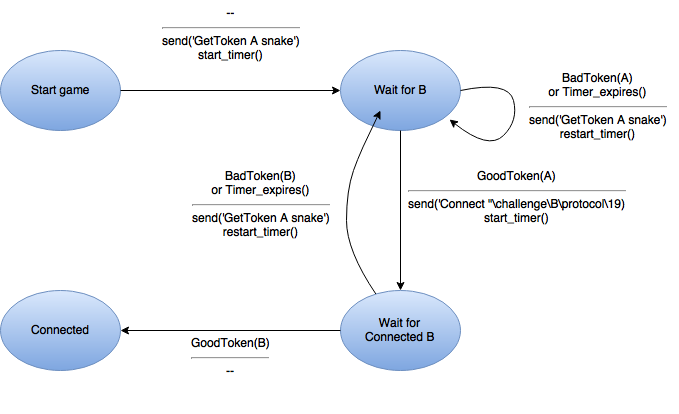
\includegraphics[scale=0.7]{sc_emetteur.png}
\end{center}
\subsection{SnakeChannel récepteur}
\begin{center}
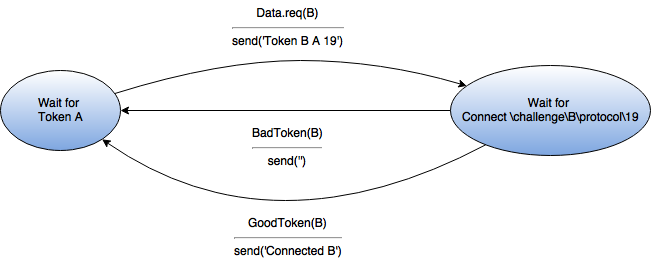
\includegraphics[scale=0.7]{sc_recepteur.png}
\end{center}
\newpage
\subsection{SnakePost émetteur}
\begin{center}
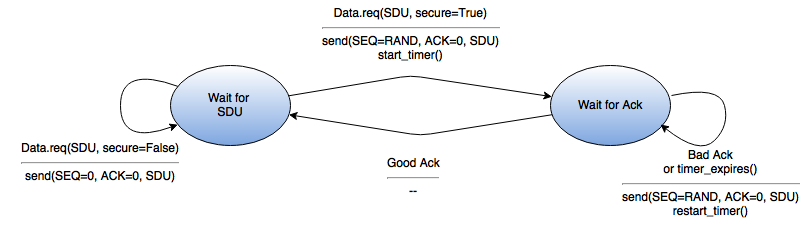
\includegraphics[scale=0.6]{sp_emetteur.png}
\end{center}
\subsection{SnakePost récepteur}
\begin{center}
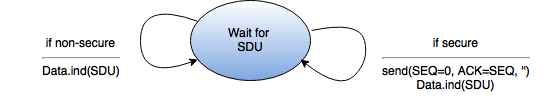
\includegraphics[scale=0.7]{sp_recepteur.png}
\end{center}
\subsection{SnakeGame joueur}
\subsubsection{Actions lors de messages reçus}
\textbf{Foods}
\begin{itemize}
\item Met à jour la position des pommes.
\end{itemize}
\textbf{Game\_over}
\begin{itemize}
\item Si le joueur est concerné, il réinitialise son serpent
\item Le statut Ready du joueur en "Game Over" est mis à False
\end{itemize}
\textbf{Grow}
\begin{itemize}
    \item Si le joueur est concerné, il augmente la taille de son serpent
\end{itemize}
\textbf{Players\_info}
\begin{itemize}
    \item Si c'est un nouveau joueur, on l'ajoute dans notre liste de serpent
    \item Sinon on modifie son score et/ou son statut
\end{itemize}
\textbf{Snakes}
\begin{itemize}
    \item On vérifie si un serpent n'est plus dans la liste pour l'enlever de notre liste de serpents
    \item Pour chaque serpent dans la liste reçu, on met à jour notre liste de serpents
\end{itemize}
\subsubsection{Messages envoyés et causes}
\textbf{Body\_p}
\begin{itemize}
\item A chaque mouvement du serpent
\end{itemize}

\textbf{Ready}
\begin{itemize}
\item A chaque pressage de la touche espace
\end{itemize}

\subsection{SnakeGame serveur}
\subsubsection{Actions lors de messages reçus}
\textbf{Body\_p}
\begin{itemize}
\item Met à jour la position du serpent
\item Si le serpent est Ready, on vérifie s'il a mangé une pomme
\item Si le serpent est Ready, on vérifie s'il n'entre pas en collision avec un autre serpent ou lui-même
\end{itemize}
\textbf{Ready}
\begin{itemize}
\item On met à True le status du serpent
\end{itemize}

\subsubsection{Messages envoyés et causes}
\textbf{Foods}
\begin{itemize}
\item Lors d'une création d'une pomme
\item Si un serpent a mangé une pomme
\item Au nouveau joueur lorsque ce dernier se connecte
\end{itemize}
\textbf{Game\_over}
\begin{itemize}
\item Si une collision se produit
\end{itemize}
\textbf{Grow}
\begin{itemize}
    \item Lorsqu'un serpent a mangé une pomme
\end{itemize}
\textbf{Players\_info}
\begin{itemize}
    \item Si une nouvelle connexion intervient
    \item A la suite d'une collision, pour la mise à jour du score
    \item Lorsqu'un joueur devient True dans Ready
\end{itemize}
\textbf{Snakes}
\begin{itemize}
    \item Si le Timer pour l'envoi des positions est échu
\end{itemize}

\section{Différences entre versions}
\subsection{Snake Channel}
La première version rendue a été complètement revu.
Au début, la logique de connexion se situait au niveau de l'application serveur et non au niveau du protocole.
La plus grosse modification est donc l'implémentation de la logique de connexion au sein du protocole, les fonctions d'envoi et de réception sont elles, restées presque inchangée.
\subsection{Snake Post}
La partie du Snake Post est quant à elle très semblable à la version finale. Nous avons modifié quelques petits bugs d'implémentation mais rien de bien méchant.

\section{Tests}
Chaque package contient un client et serveur test permettant de tester le protocole sans le jeu Snake.
Le package Snake Post en contient deux pour pouvoir tester l'implémentation sur UDP et sur Snake Channel.

\end{document}
